\chapter{Antecedentes en el an\'alisis de rendimiento en Hyperledger Fabric}\label{chapter:state-of-the-art}

Los estudios a las versiones m\'as recientes de Hyperledger Fabric se remontan a noviembre del 2020, cuando el laboratorio de tecnolog\'ia RF y comunicaciones m\'oviles de la Universidad de Ciencias Aplicadas de Osnabrück en Alemania realiz\'o un estudio al rendimiento de la plataforma en su versi\'on 2.0, estrenada en febrero de ese mismo a\~no [\cite{dreyer2020performance}].\\

El prop\'osito de ese trabajo fue obtener una evaluaci\'on definitiva de c\'omo la variaci\'on de los diferentes participantes de la red influyen en su rendimiento. En particular, el n\'umero de nodos pares, organizaciones, nodos ordenadores y el tama\~no de los bloques. Julian Dreyer desarroll\'o una herramienta [\cite{Configurator}] para Fabric 2.0 que genera autom\'aticamente la red requerida con el n\'umero deseado de componentes e instala el contrato inteligente de prueba. Las m\'etricas de rendimiento no se miden directamente, sino emplearon f\'ormulas para obtenerlas:\\

\emph{Rendimiento} $ = \frac{1s}{\frac{ \sum_i^N t\_tx_i } {N} }$ [TPS]\\

\emph{Tasa de Error} $ = \frac{F}{N} \cdot 100\% $\\


\emph{Latencia} $ = t\_tx_i + t\_b_i$ [ms]

{\vspace{1 cm}}

donde:
\begin{itemize}
\item $t\_tx_i$ es el tiempo de la i-\'esima transacci\'on.
\item $t\_b_i$ es el tiempo de confirmaci\'on del i-\'esimo bloque.
\item $F$ denota el n\'umero de transacciones fallidas.
\item $N$ el total de transacciones efectuadas.  
\end{itemize}

El estudio se realiz\'o en un sistema operativo Ubuntu 16.04 con dos CPU Intel Xeon E5-2690 y 128GB 2133MHz RAM. Se utiliz\'o Docker 19.03.8 para las im\'agenes de Fabric 2.0.\\

Las configuraciones empleadas para la red de Fabric se muestran en la tabla \ref{tab:Configuraciones} y siguen un esquema abreviado: \texttt{<organizaciones>-<pares>-<ordenadores>-<nodos-kafka>}. Para los esquemas de pruebas individuales en cada tasa de transacci\'on se utiliza la notaci\'on: \texttt{ bs<tama\~no de los bloques>-<transacciones por segundos>tps}.\\

En los escenarios de prueba, todos los pares configurados est\'an asignados para cumplir con la pol\'itica de aprobaci\'on.\\

Primero fijaron el n\'umero de nodos ordenadores, nodos kafka y organizaciones en uno, para garantizar un entorno de referencia y escalar los nodos pares comenzando con solo dos hasta llegar a diecis\'eis por organizaci\'on. La Figura \ref{EscalaParesUnaOrganizacion} muestra gr\'aficamente los tiempos de ejecuci\'on para cada configuraci\'on. El eje x tambi\'en incluye las variaciones en el tama\~no de los bloques y las \emph{TPS}.\\

\begin{figure}[h]
\centering
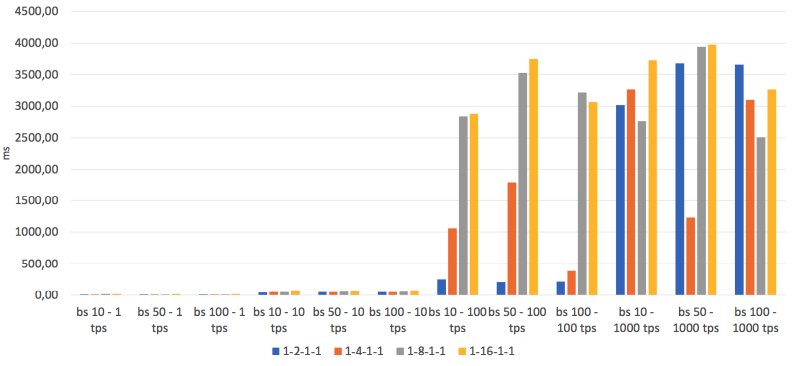
\includegraphics[width=0.6\linewidth]{Graphics/EscalaParesUnaOrganizacion.png}
\caption{Tiempo de ejecuci\'on en una organizaci\'on. \emph{Fuente: Performance analysis of hyperledger fabric 2.0 blockchain platform.}}
\label{EscalaParesUnaOrganizacion}
\end{figure}

Al aumentar la cantidad de nodos pares dentro de una organizaci\'on, se percibe un aumento significativo en el tiempo de ejecuci\'on de la transacci\'on. La introducci\'on de m\'as nodos pares conduce a una mayor sobrecarga de comunicaci\'on y sincronizaci\'on dentro de la red. Al analizar el mismo escenario con dos organizaciones, la tendencia general con respecto al impacto en el rendimiento contin\'ua. En el caso de los tiempos de ejecuci\'on, la configuraci\'on con dos organizaciones, produce tiempos en las transacciones m\'as bajos en promedio. Sin embargo, esta tendencia particular no contin\'ua cuando se considera la misma configuraci\'on con cuatro organizaciones. Los resultados tienen una mayor similitud a los de la figura \ref{EscalaParesUnaOrganizacion}, lo que sugiere una optimizaci\'on de los tiempos de transacci\'on para dos organizaciones. Nasir en [\cite{nasir2018performance}] hab\'ia observado igual comportamiento para versiones anteriores de Fabric.\\

El impacto negativo en el aumento del n\'umero de pares tambi\'en influye en los tiempos de confirmaci\'on de los bloques. La Figura \ref{BlockCommit} muestra los tiempos de confirmaci\'on de los bloques para cada caso de prueba en una organizaci\'on.\\

\begin{figure}[h]
\centering
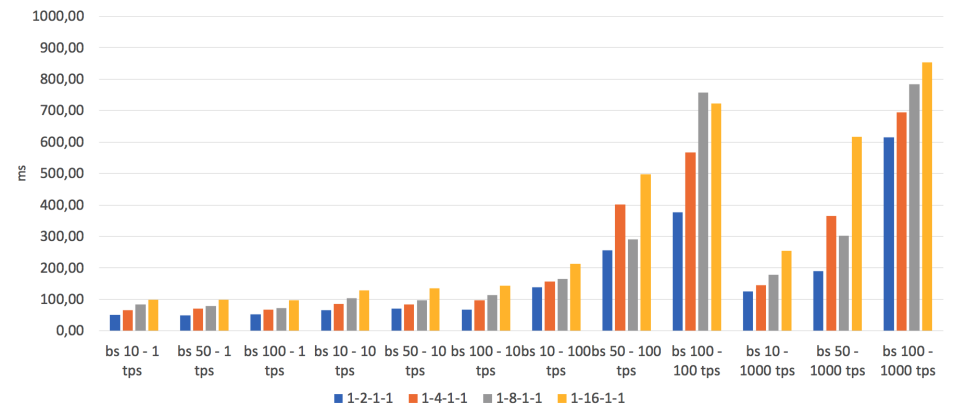
\includegraphics[width=0.6\linewidth]{Graphics/BlockCommit.png}
\caption{Tiempo de confirmaci\'on de bloques en una organizaci\'on. \emph{Fuente: Performance analysis of hyperledger fabric 2.0 blockchain platform.}}
\label{BlockCommit}
\end{figure}

Con respecto a la tasa de error, se muestra generalmente creciente con TPS m\'as elevadas como se observa en la figura \ref{ErrorRate}. Sin embargo, un tama\~no de bloque mayor tiene un efecto positivo, en promedio, en la tasa de error. Causando menos errores en tiempo de ejecuci\'on.\\

\begin{figure}[h]
\centering
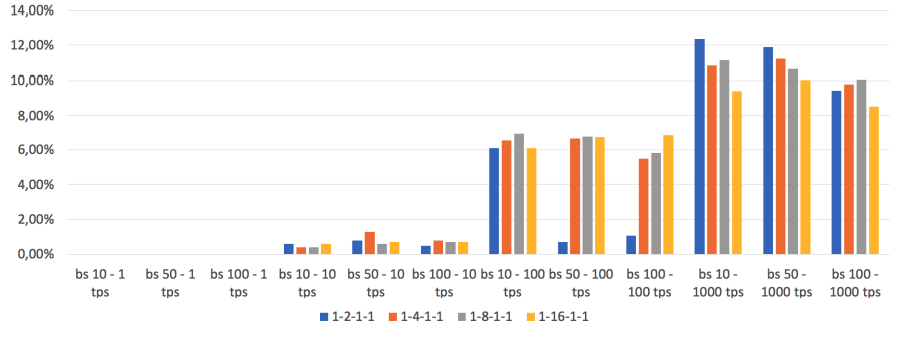
\includegraphics[width=0.6\linewidth]{Graphics/ErrorRate.png}
\caption{Tasa de error en una organizaci\'on. \emph{Fuente: Performance analysis of hyperledger fabric 2.0 blockchain platform.}}
\label{ErrorRate}
\end{figure}

El servicio de ordenaci\'on no ejecuta transacciones, por tanto, es de esperar que al escalar los nodos ordenadores apenas afecten los tiempos en las transacciones. Aunque, si deben influir en los tiempos de confirmaci\'on de los bloques. Un aumento en el n\'umero de nodos ordenadores requiere una mayor sincronizaci\'on entre ellos, que se refleja en el rendimiento de la red.\\

Las pruebas realizadas para comprobar el impacto de la variaci\'on del n\'umero de nodos ordenadores no arrojaron un resultado generalizable, como en el caso de los nodos pares. Se puede apreciar en las figuras \ref{BlockCommitOrderes} y \ref{EscalaOrderesCuatroOrganizacion} .\\

\begin{figure}[h]
\centering
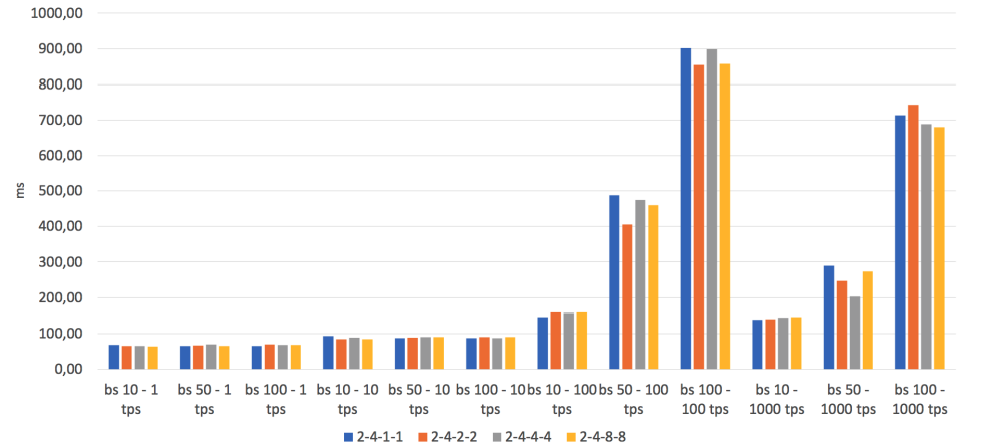
\includegraphics[width=0.6\linewidth]{Graphics/BlockCommitOrderes.png}
\caption{Tiempo de confirmaci\'on de bloques en dos organizaci\'on. \emph{Fuente: Performance analysis of hyperledger fabric 2.0 blockchain platform.}}
\label{BlockCommitOrderes}
\end{figure}

\begin{figure}[h]
\centering
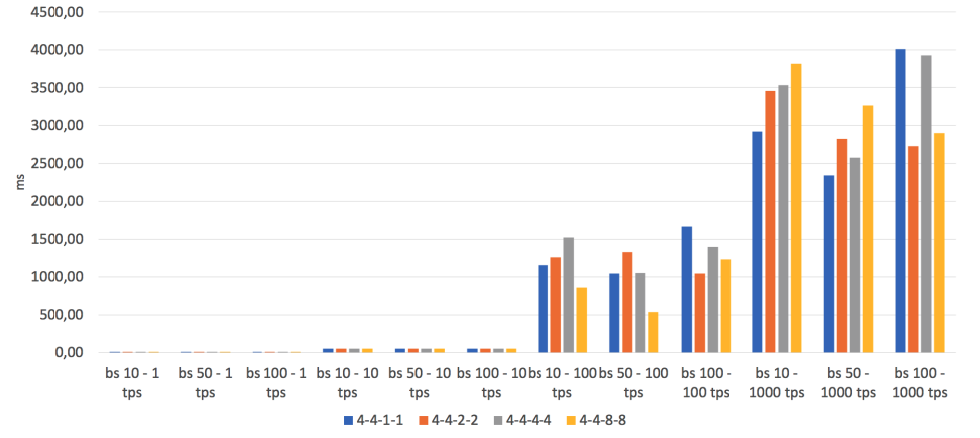
\includegraphics[width=0.6\linewidth]{Graphics/EscalaOrderesCuatroOrganizaciones.png}
\caption{Tiempo de ejecuci\'on en cuatro organizaci\'on. \emph{Fuente: Performance analysis of hyperledger fabric 2.0 blockchain platform.}}
\label{EscalaOrderesCuatroOrganizacion}
\end{figure}

Se confirma que a mayor tama\~no de bloques, mayor ser\'a su tiempo de confirmaci\'on en el \emph{ledger}. Debido a que se incluyen m\'as transacciones y, por lo tanto, requiere m\'as tiempo para validarlas. Esto conduce a que el tama\~no del bloque est\'a en correlaci\'on directa con la latencia global del sistema.\\

En resumen, el rendimiento depende en gran medida de la cantidad de nodos pares. M\'as nodos pares de respaldo activos dentro de la red ocasiona menor rendimiento. En el caso de la latencia depende, tanto del tama\~no del bloque, como de la cantidad de nodos pares de aprobaci\'on. Cuando el tama\~no de los bloques es peque\~no, generalmente permite una latencia menor. Sin embargo, debe seleccionarse en funci\'on de la tasa de \emph{TPS} esperada porque un llenado r\'apido de los bloques puede resultar en un proceso de validaci\'on frecuente. Se afirma adem\'as que solo el tama\~no de los bloques y la tasa de \emph{TPS} tienen una influencia marcada en la tasa de error. Un tama\~no de bloque m\'as grande producir\'a menos errores que uno m\'as peque\~no.